\chapter{Final Implementation}
\label{chapter:implementation}

%----------------------------------------------------------------------------------------
%	Section
%----------------------------------------------------------------------------------------

\section{Final System on DSP Board}
The final system implemented on ADSP-BF548 realizes following functions.
\begin{itemize}
\item Adaptive noise cancellation based on Least Mean Square Algorithm
\item Real-time recognition of spoken words
\item Result indication via a five-LED array
\item YouTube controller
\end{itemize}

\subsection{LED Indicator}
In addition to the result sent back to VisualDSP++, LEDs are employed to indicate recognition result. The DSP board provides 6 general-purpose (\textcolor{orange_html}{amber}) LEDs. \texttt{LED1} through \texttt{LED6} are accessed via the \texttt{PG6}-\texttt{PG11} pins of the processor \cite{bf548-manual}.\\

As is summarized in Table \ref{table 1} on page \pageref{table 1}, there are 27 potential recognition outcomes. \texttt{LED1} to \texttt{LED5} with a capacity of $2^5 = 32$ are designed to represent the recognition result and \texttt{LED6} toggles between `on' and `off' when new result comes. For example, \LED\onLED\offLED\onLED\offLED\onLED\ represents word \textit{zero} ($(10101)_2 = 21$) while \LED\offLED\onLED\offLED\onLED\offLED\ symbolizes word \textit{ten} ($(01010)_2 = 10$). Five zeros \LED\offLED\offLED\offLED\offLED\offLED\ mean invalid recognition outcomes.

\subsection{Utilization in Home Automation}
We use an Arduino\textsuperscript{\textregistered} board as an intermediate between the word recognition system and applications in home automation primarily because of the open-source ecosystem of abundant resources already available to Arduino developers. For example, with the aid of infrared emitter and WIFI module as well as supporting example program, we are able to easily control a TV and send command via wireless communication.

\subsubsection{Communication between DSP and Arduino}
We simply utilize general purpose input / output (GPIO) pins to exchange information between DSP and Arduino. \texttt{PG6}-\texttt{PG11} pins connected to \texttt{LED1}-\texttt{LED6} are accessible through pin 79-84 of \texttt{J1} connector on the back of DSP board. (Fig. \ref{J1-schematic} on page \pageref{J1-schematic} illustrates the pin information of \texttt{J1} connector.) Five TTL values (either `high' or `low') encode the recognition outcome and the toggle of most significant bit indicates the advent of new result.\\

We also tried to transmit command via UART serial port. It took a long time to configure the corresponding device manager. Eventually, we decided to stick on the GPIO method.

\subsubsection{Communication between Arduino and PC}
Arduino retrieves logic levels of aforementioned pins and then decodes the binary information. At the next step, Arduino sends the decoded result to the WIFI module via the serial port (8 data bits, no parity, one stop bit, 9600 bps). At this stage, PC can directly receive the result through a USB cable.

\subsubsection{YouTube Controller on PC}
A python program keeps listening the serial port (wired connection) or the \texttt{Telnet} port (wireless connection). Afterwards, python program simulates a keyboard press according to the received command. Thereby, YouTube on TV becomes controlled by speech command.

\subsubsection{Other applications}
Thanks to the ample Arduino accessories, more home appliances can be easily integrated into our system. For example, air conditioners can be controlled by the infrared signal sent by IR emitter. AC lights can also be controlled by an Arduino with relay module.

\begin{figure}[H]
\centering
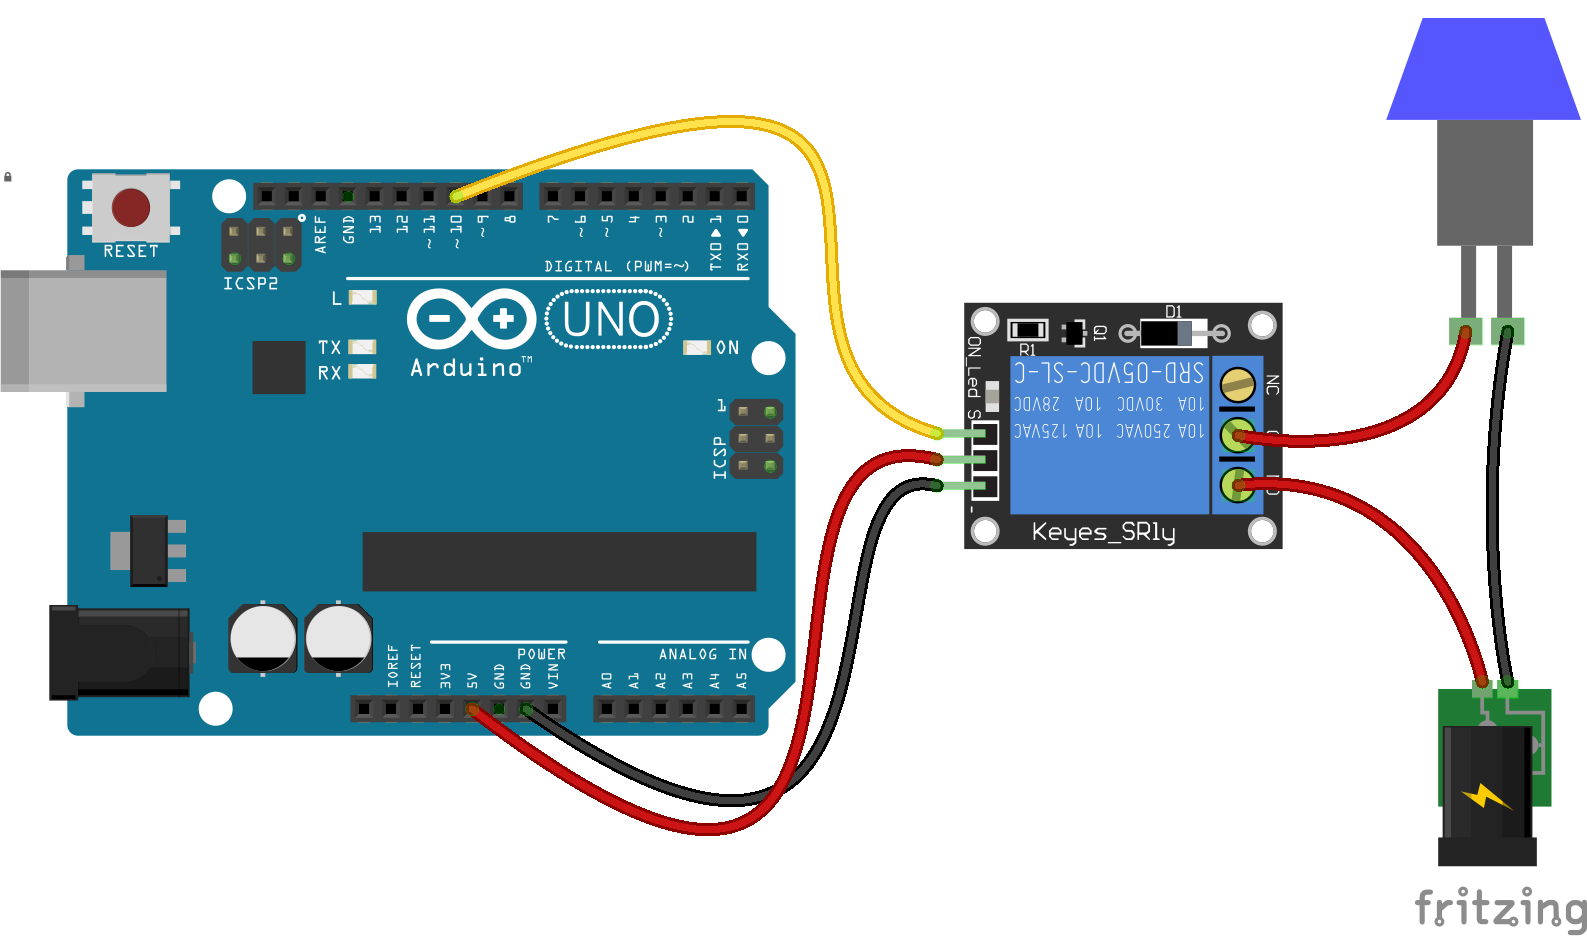
\includegraphics[width=3in]{ang/relay-arduino}
\caption{Control AC Light using Arduino with Relay Module \cite{relay-arduino}}
\label{relay-arduino}
\end{figure}

%----------------------------------------------------------------------------------------
%	Section
%----------------------------------------------------------------------------------------

\section{Performance on DSP board}

\subsection{Feature Extraction \& Recognition}

We randomly test the final system on DSP for 23 times and compare the outcomes computed by DSP and MATLAB. In term of dataset $n$ ($n = 1, 2, \dots, 23$) and word $k$ ($k = 1, 2, \dots, 27$), let $p_{MATLAB}[n, k]$ denote the probability (natural-log scale) computed by MATLAB and $p_{DSP}[n, k]$ denote the probability (natural-log scale) computed by DSP.\\

We define the \textit{relative error} of word $k$ in dataset $n$
\begin{equation}
\varepsilon[n, k] = \frac{p_{DSP}[n, k] - p_{MATLAB}[n, k]}{p_{MATLAB}[n, k]}
\end{equation}
and the \textit{Root Mean Square Error} of dataset $n$
\begin{equation}
\epsilon_{RMSE}[n] = \sqrt{\frac{1}{27} \sum_{k = 1}^{27} (\varepsilon[n, k])^2}
\end{equation}
For a certain dataset $n$, $\epsilon_{RMSE}[n]$ represents the `average' of $\varepsilon[n, k]$.\\

Fig. \ref{relative_error} shows that absolute relative error $|\varepsilon[n, k]|$ ranges from $1 \times 10^{-6}$ to $9 \times 10^{-3}$ and dataset 1 has the largest deviation (\textcolor{navy_matlab}{navy solid line}). Fig. \ref{root_mean_square_error} illustrates the root mean square error $\epsilon_{RMSE}[n]$ of each dataset $n$ and dataset 1 has the largest $\epsilon_{RMSE}[n]$ consistently (\textcolor{navy_matlab}{navy solid line}).

\begin{figure}[H]
\begin{minipage}[t]{0.5\linewidth}
\centering
\minipageplot{ang/relative_error}
\caption{$\varepsilon[n, k]$ of 27 words in 23 datasets}
\label{relative_error}
\end{minipage}
\begin{minipage}[t]{0.5\linewidth}
\centering
\minipageplot{ang/root_mean_square_error}
\caption{$\epsilon_{RMSE}[n]$ of 27 words}
\label{root_mean_square_error}
\end{minipage}
\end{figure}

In fact, the computation error has no influence on recognition result. Take dataset 1 with the largest root mean square error as an example, Fig. \ref{word_probabilities} depicts the probabilities of 27 words computed by MATLAB (\textcolor{navy_matlab}{navy circle $\circ$}) and DSP (\textcolor{orange_matlab}{orange cross $\times$}). It can be clearly seen that error are much less than the differences between probabilities. Word \textit{one} can be recognized without any interference.

\begin{figure}[H]
\begin{minipage}[t]{0.5\linewidth}
\centering
\minipageplot{ang/word_probabilities}
\caption{27 probabilities in dataset 1}
\label{word_probabilities}
\end{minipage}
\begin{minipage}[t]{0.5\linewidth}
\centering
\minipageplot{ang/processing_time}
\caption{Processing time}
\label{processing_time}
\end{minipage}
\end{figure}

The clocks required to extract speech features and obtain recognition outcome are plotted in Fig. \ref{processing_time}. Given $6 \times 10^8$ clocks per second, corresponding processing time can be converted. The average processing time of these 23 datasets is \textbf{97 milliseconds}. Processing time varies because different number of frames are passed into MFCC after threshold.
